\documentclass[report.tex]{subfiles}

\externaldocument{report}

\begin{document}

\section{失敗点・言い訳}

\subsection{アンテナの作成}

\subsubsection{かご}

まず、ループアンテナを作成するときに、100円ショップで買ったかごを巻き付けて作成しようと思った(\wfig{kago})。
しかし、かごが斜めっているせいで両面テープで補強しても巻き付けた部分がどうしてもズレてしまい、作業が進まなかった。

\begin{figure}[H]
	\centering
	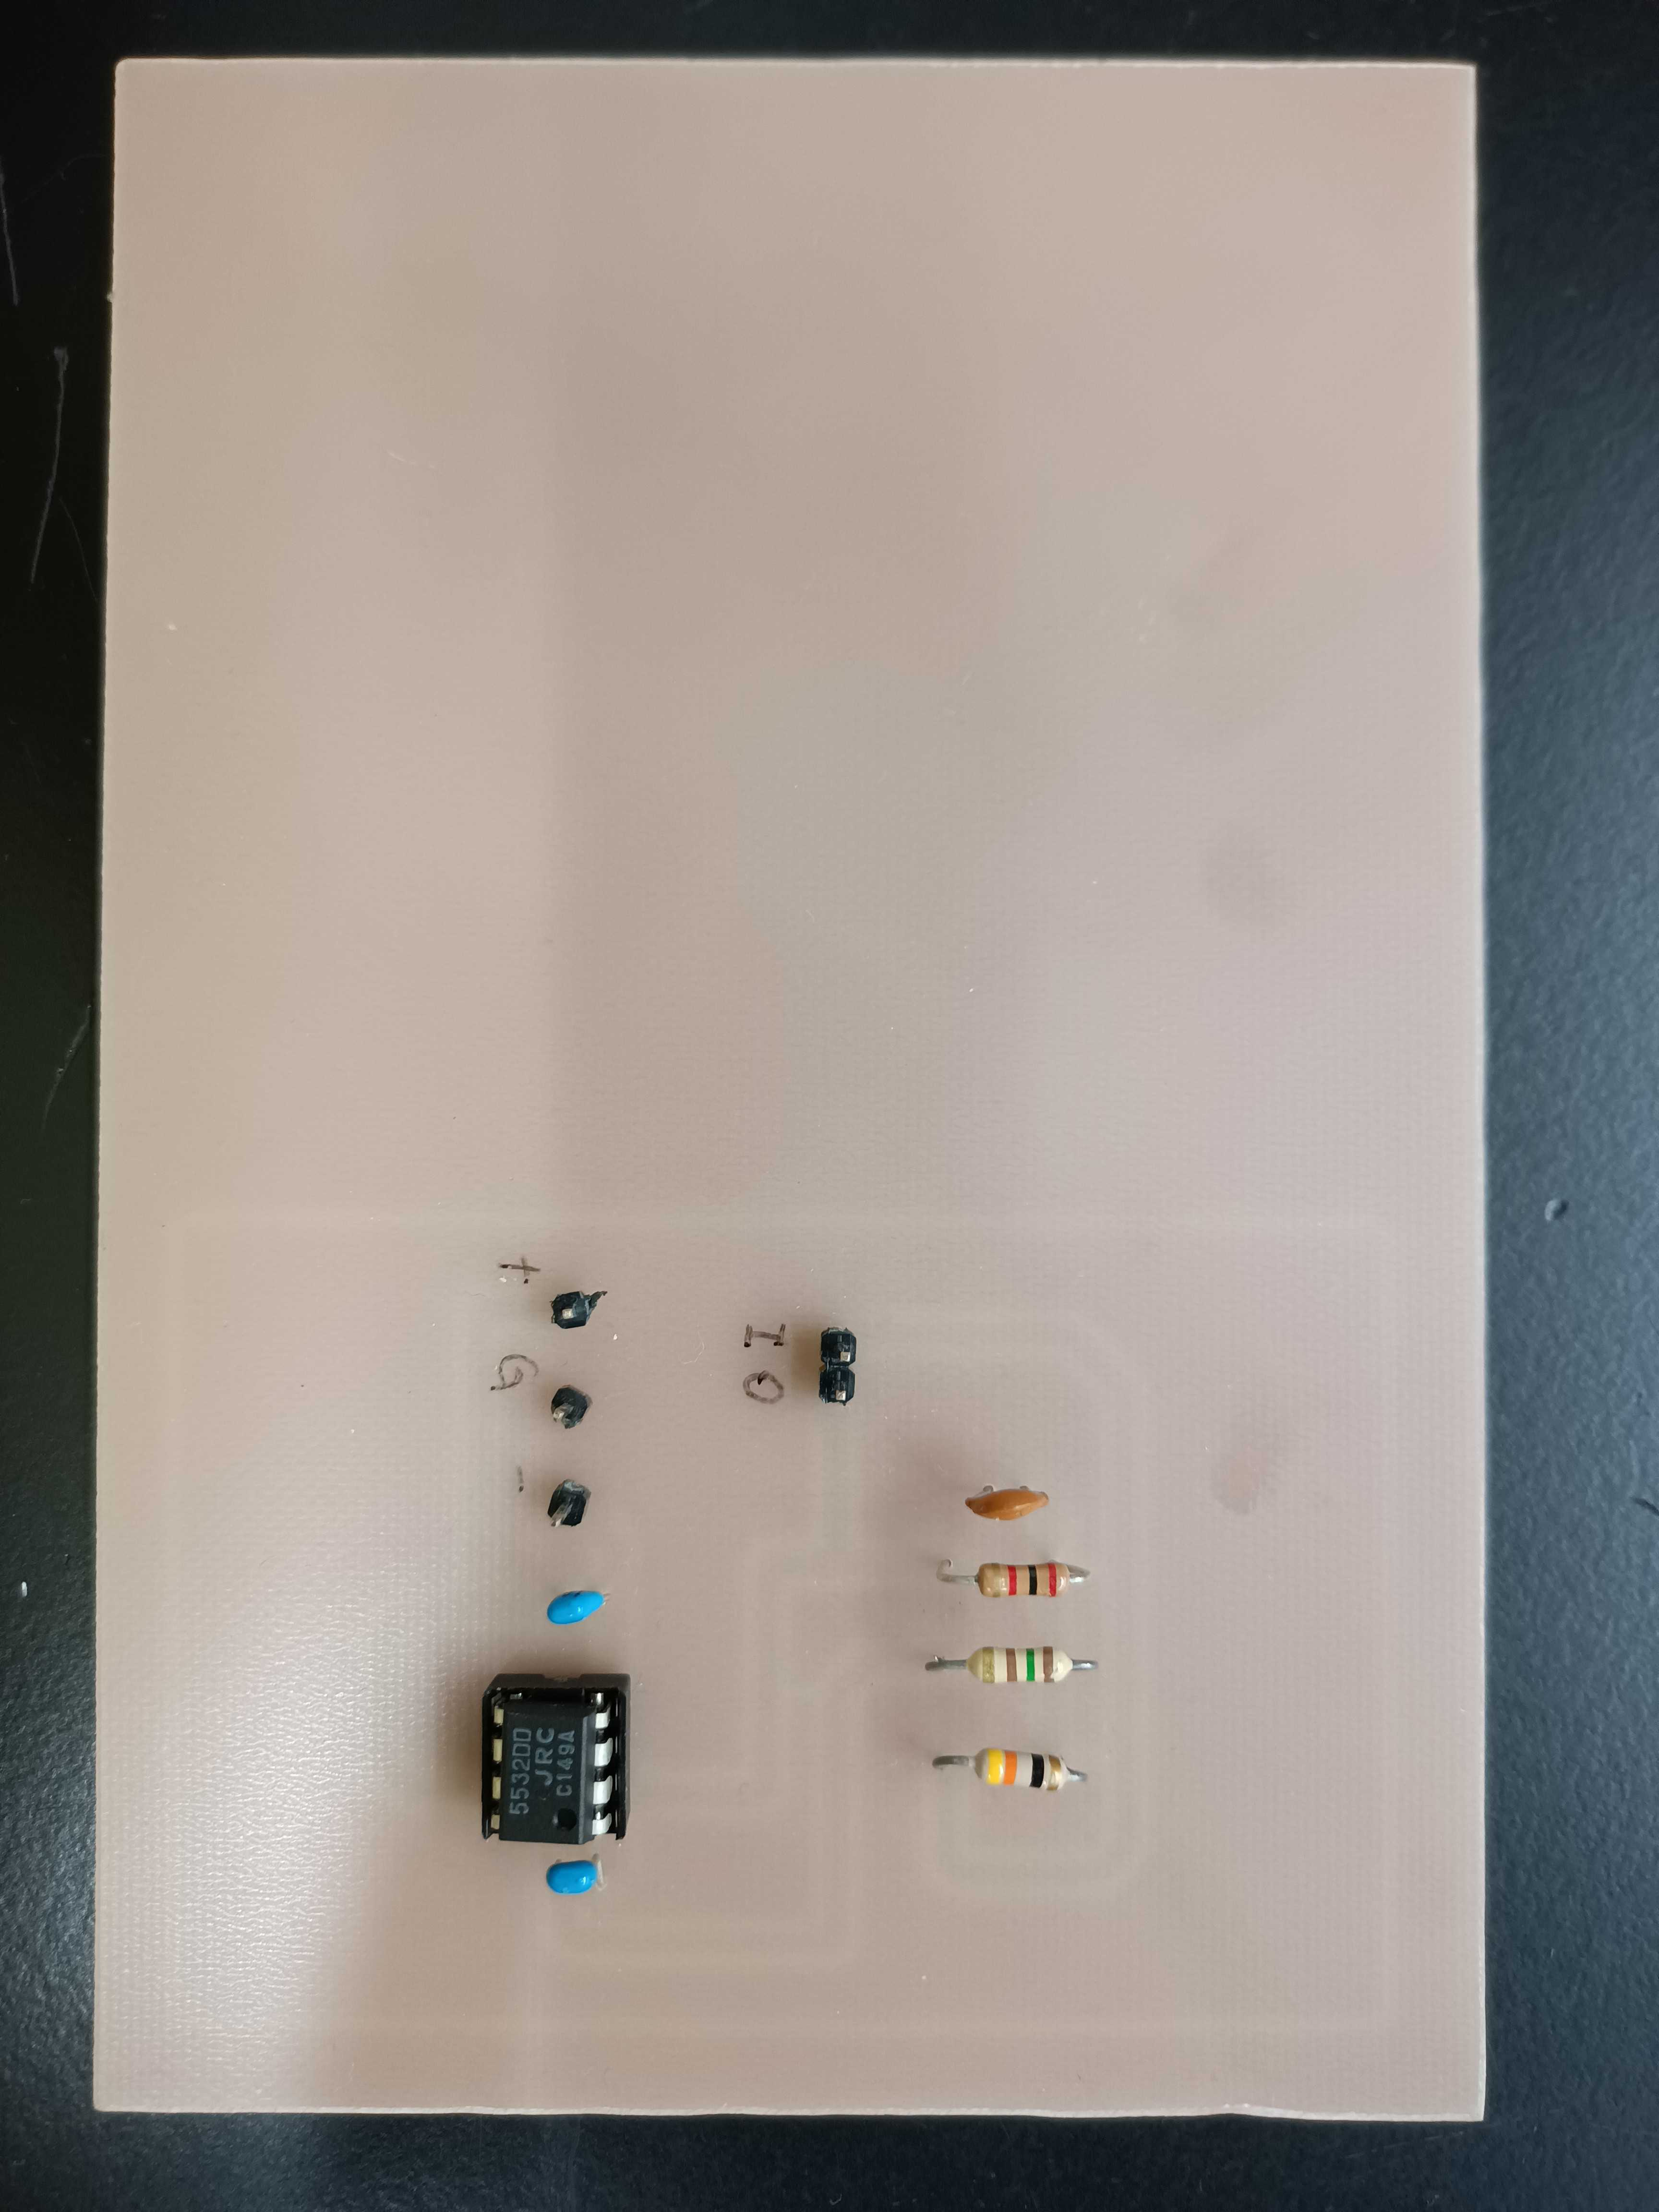
\includegraphics[width=7cm]{use/1.jpg}
	\caption{かご}
	\label{fig:kago}
\end{figure}

また、「それだとコイルが斜めっているからちゃんとアンテナとして機能しないんじゃないの?」と言われ、かごに巻き付けるのを断念した。
かごが斜めっていると、想定していたインダクタンス値からかなりズレてしまうと思った。
様々な巻数で電波の受信感度を測定できたらいいのではないかと思い、かごにドリルで穴を開けてそこから導線を通してみようと考えた。
しかし、そう思った時点では、すでにかなりの巻数を巻いてしまっていたので、穴を開けるために巻いてしまった部分をやり直したり、かごについていた出っ張りの部分が邪魔であったりして、穴を開けるのが非常に困難であったり、穴を想定よりかなりズレたところに開けてしまったりして、かごでやったのは絶対に失敗したと感じた。

\subsubsection{エナメル線}

最初に、0.32mmの導線でアンテナを巻き付ける際に、秋葉原で売っていた20mのエナメル線を用いた。
袋を開けてから、何も考えずにすぐに巻き付けようとしてしまった。そのせいでヒモがどんどんと絡まってしまった。
その時、竹中が開封したときは、きれいな導線だったから引っ張ればもとに戻ると勘違いしてしまい、他の二人がそれは良くないと言っていたが、気づいたときには、元には戻せないほど絡まってしまった。
次からは、

\subsection{増幅回路の作成}

\begin{figure}[H]
	\begin{minipage}[b]{0.5\linewidth}
		\centering
		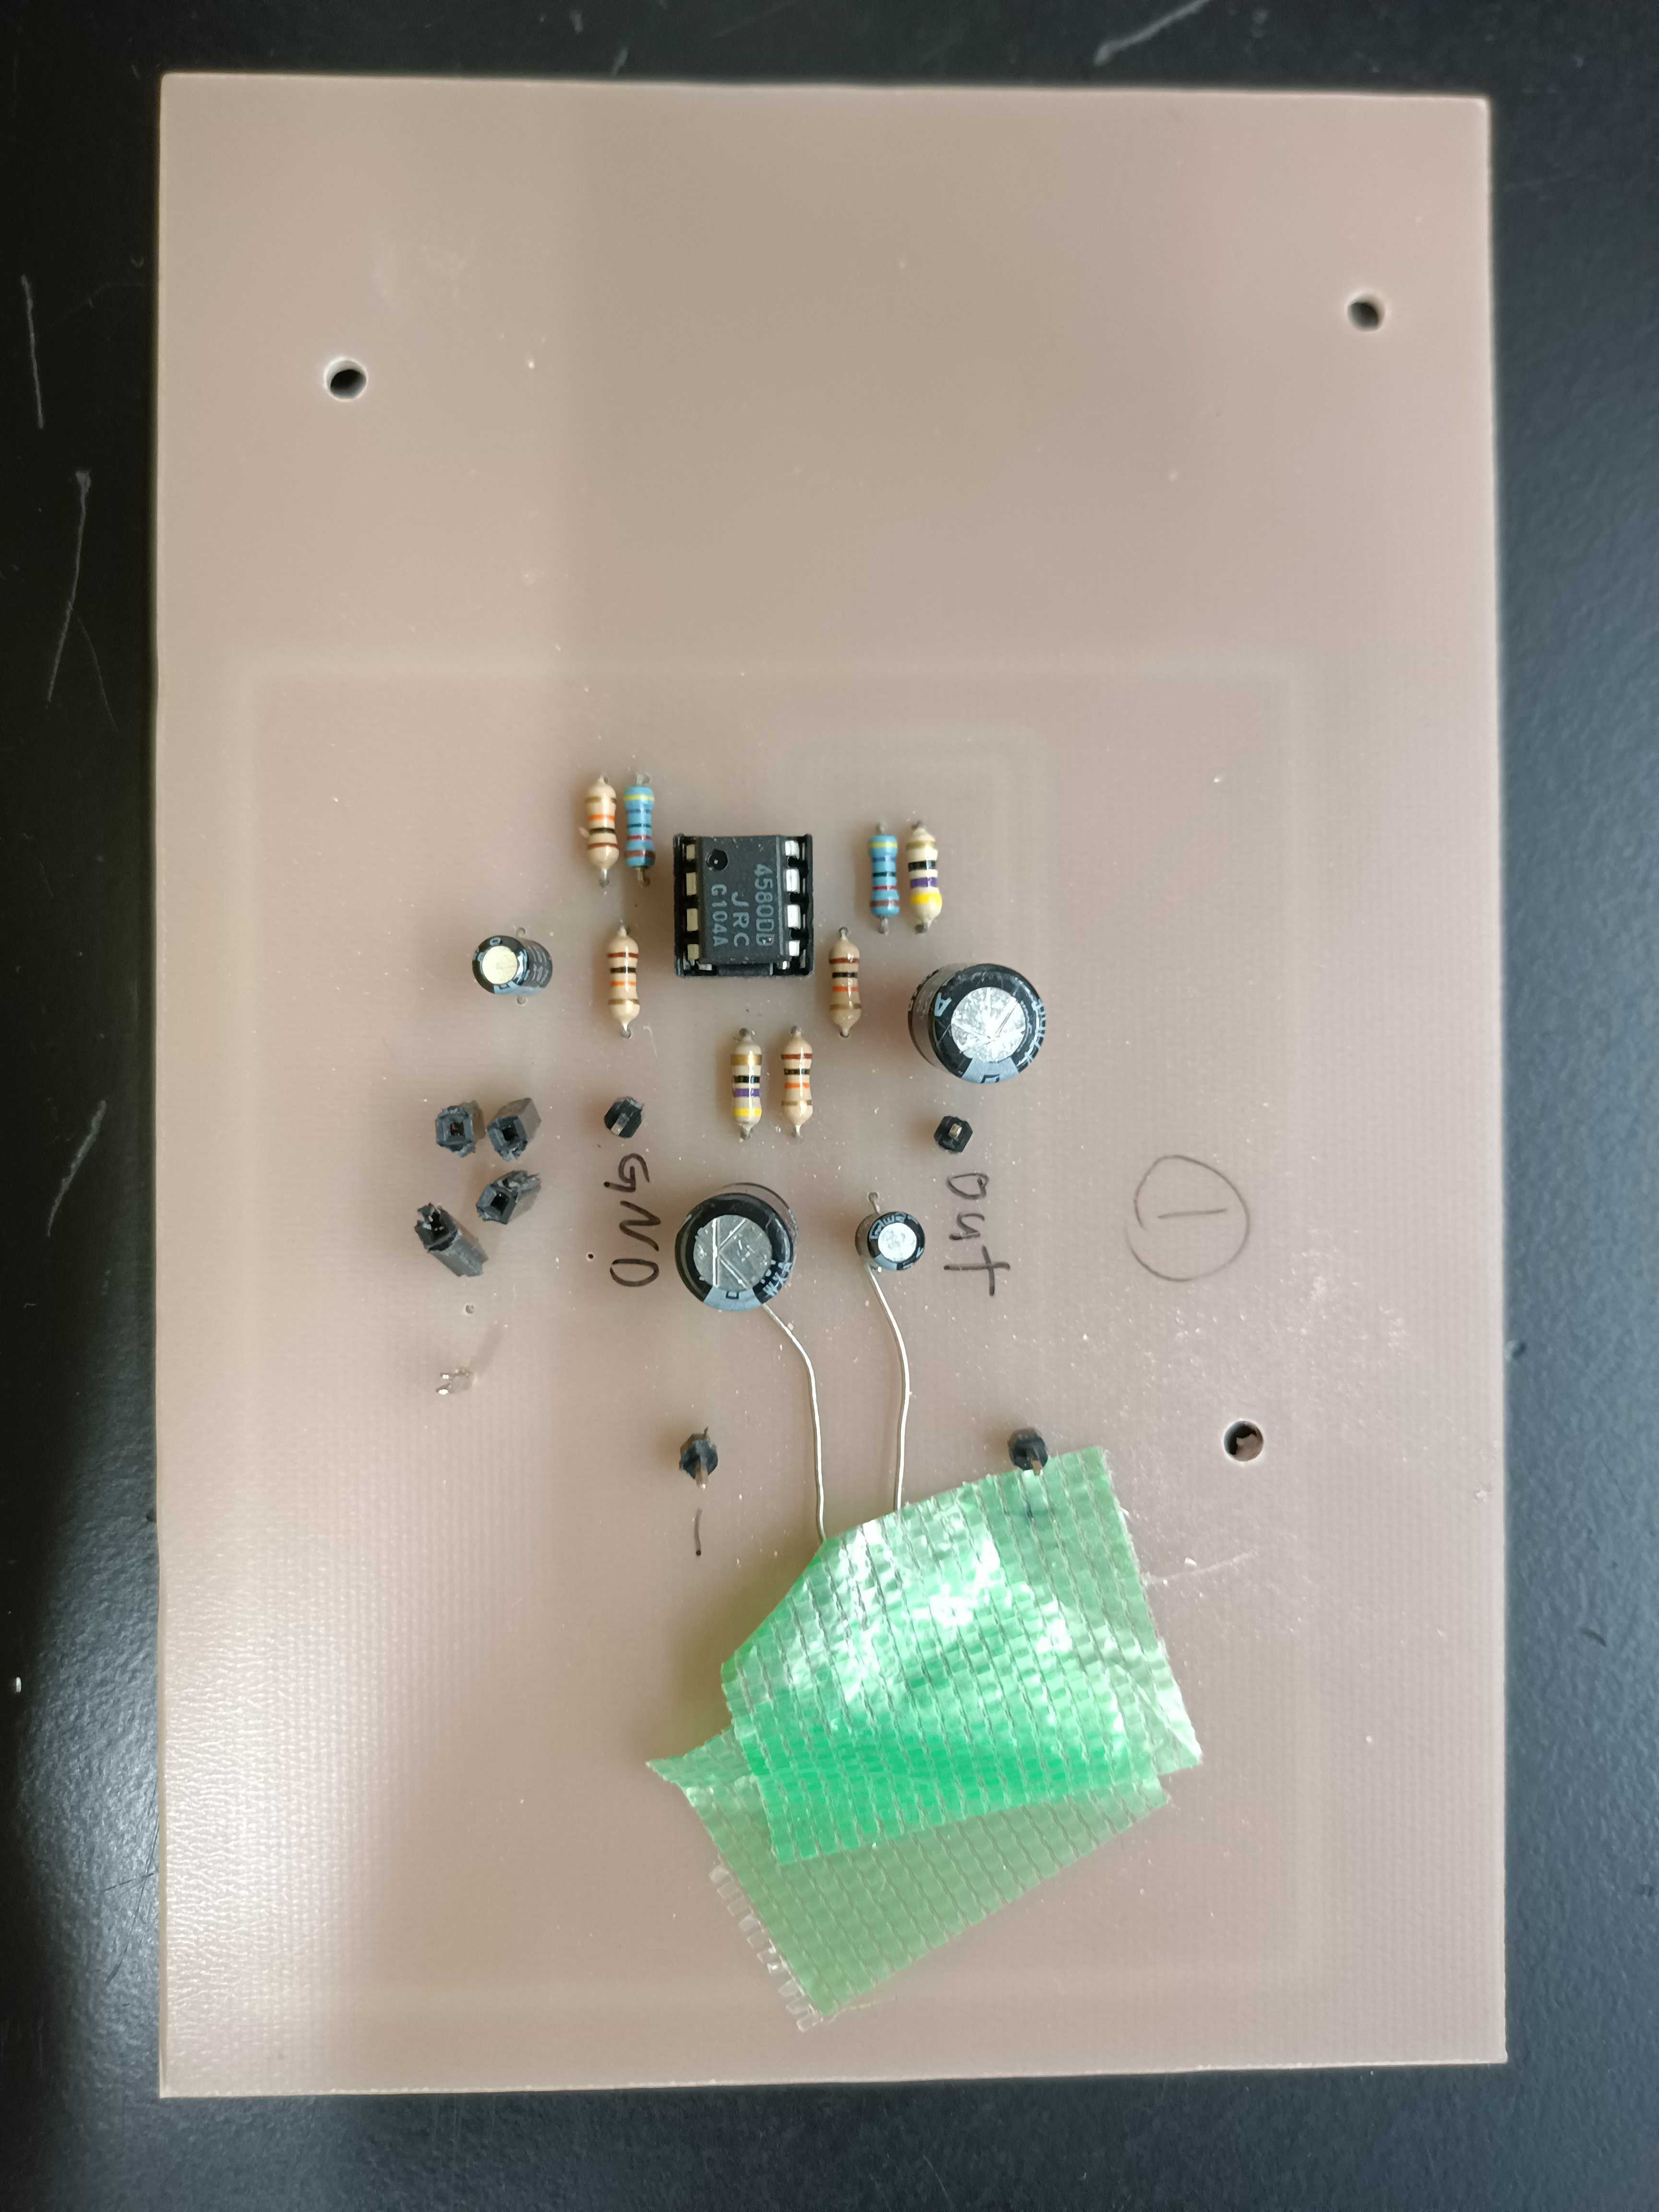
\includegraphics[width=8cm]{use/2.jpg}
		\caption{2号機アンテナの写真}
		\label{fig:s_2}
	\end{minipage}
	\begin{minipage}[b]{0.5\linewidth}
		\centering
		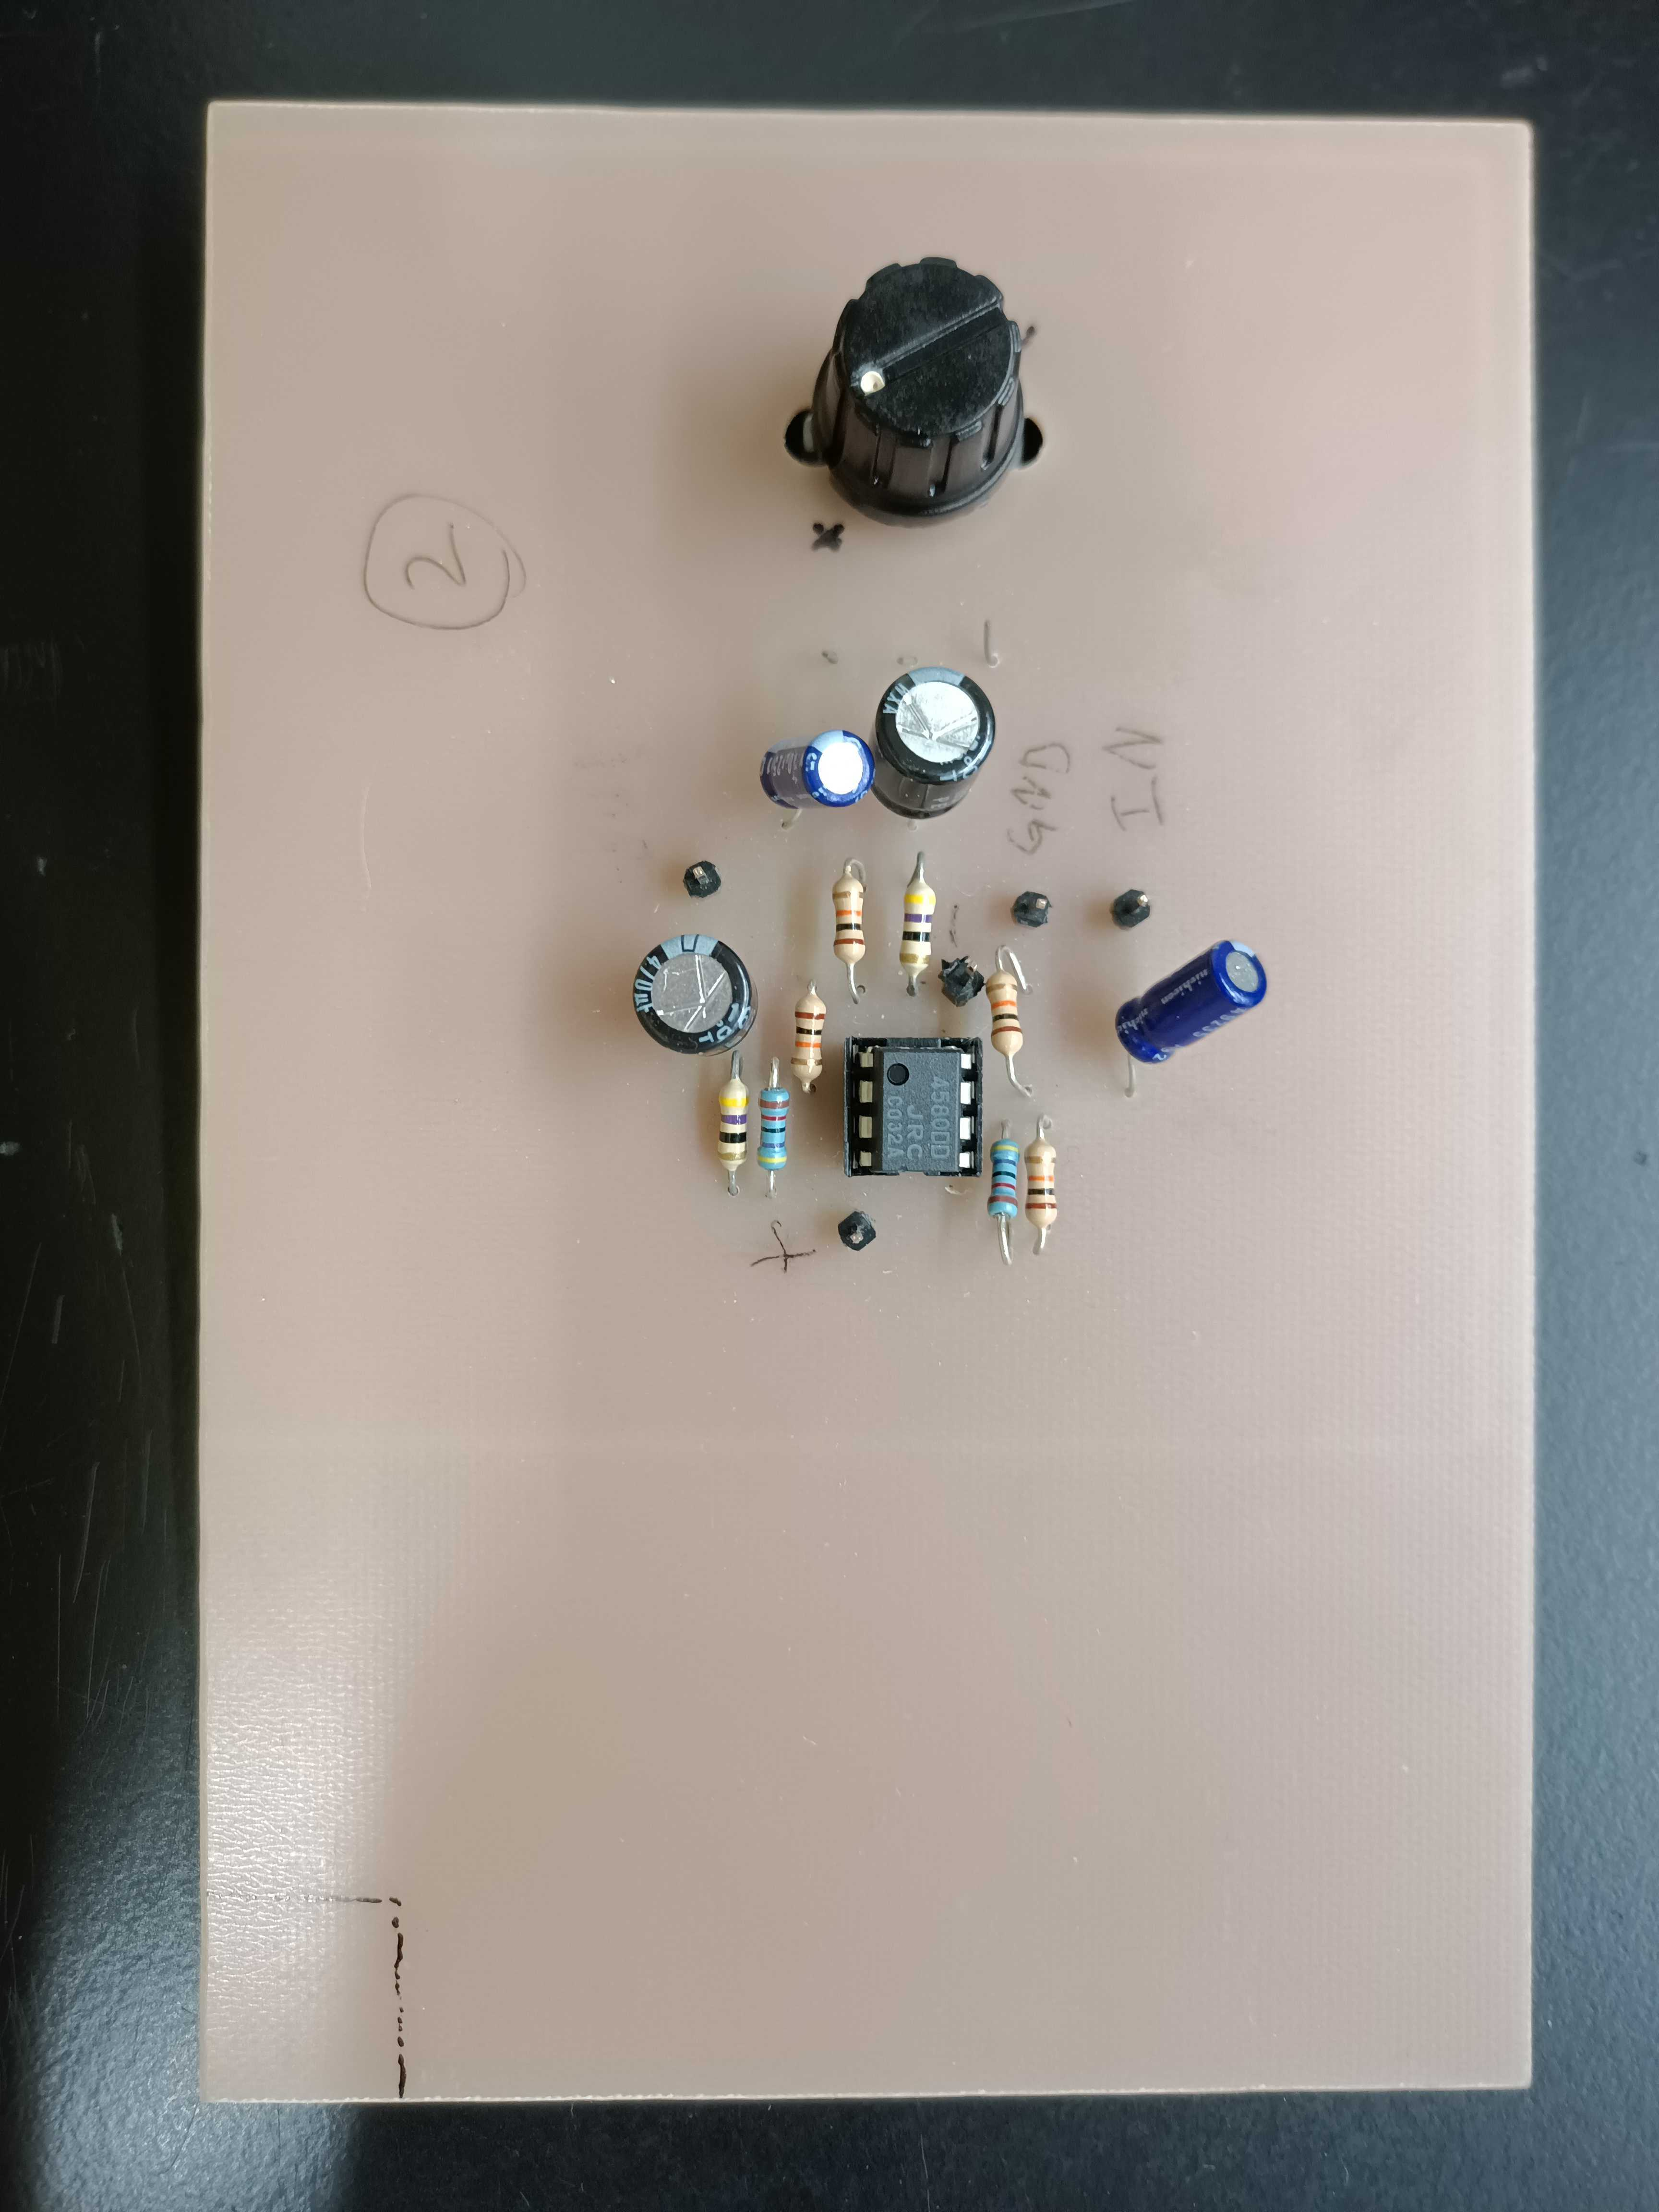
\includegraphics[width=8cm]{use/3.jpg}
		\caption{3号機アンテナの写真}
		\label{fig:s_3}
	\end{minipage}
\end{figure}

\begin{figure}[H]
	\begin{minipage}[b]{0.5\linewidth}
		\centering
		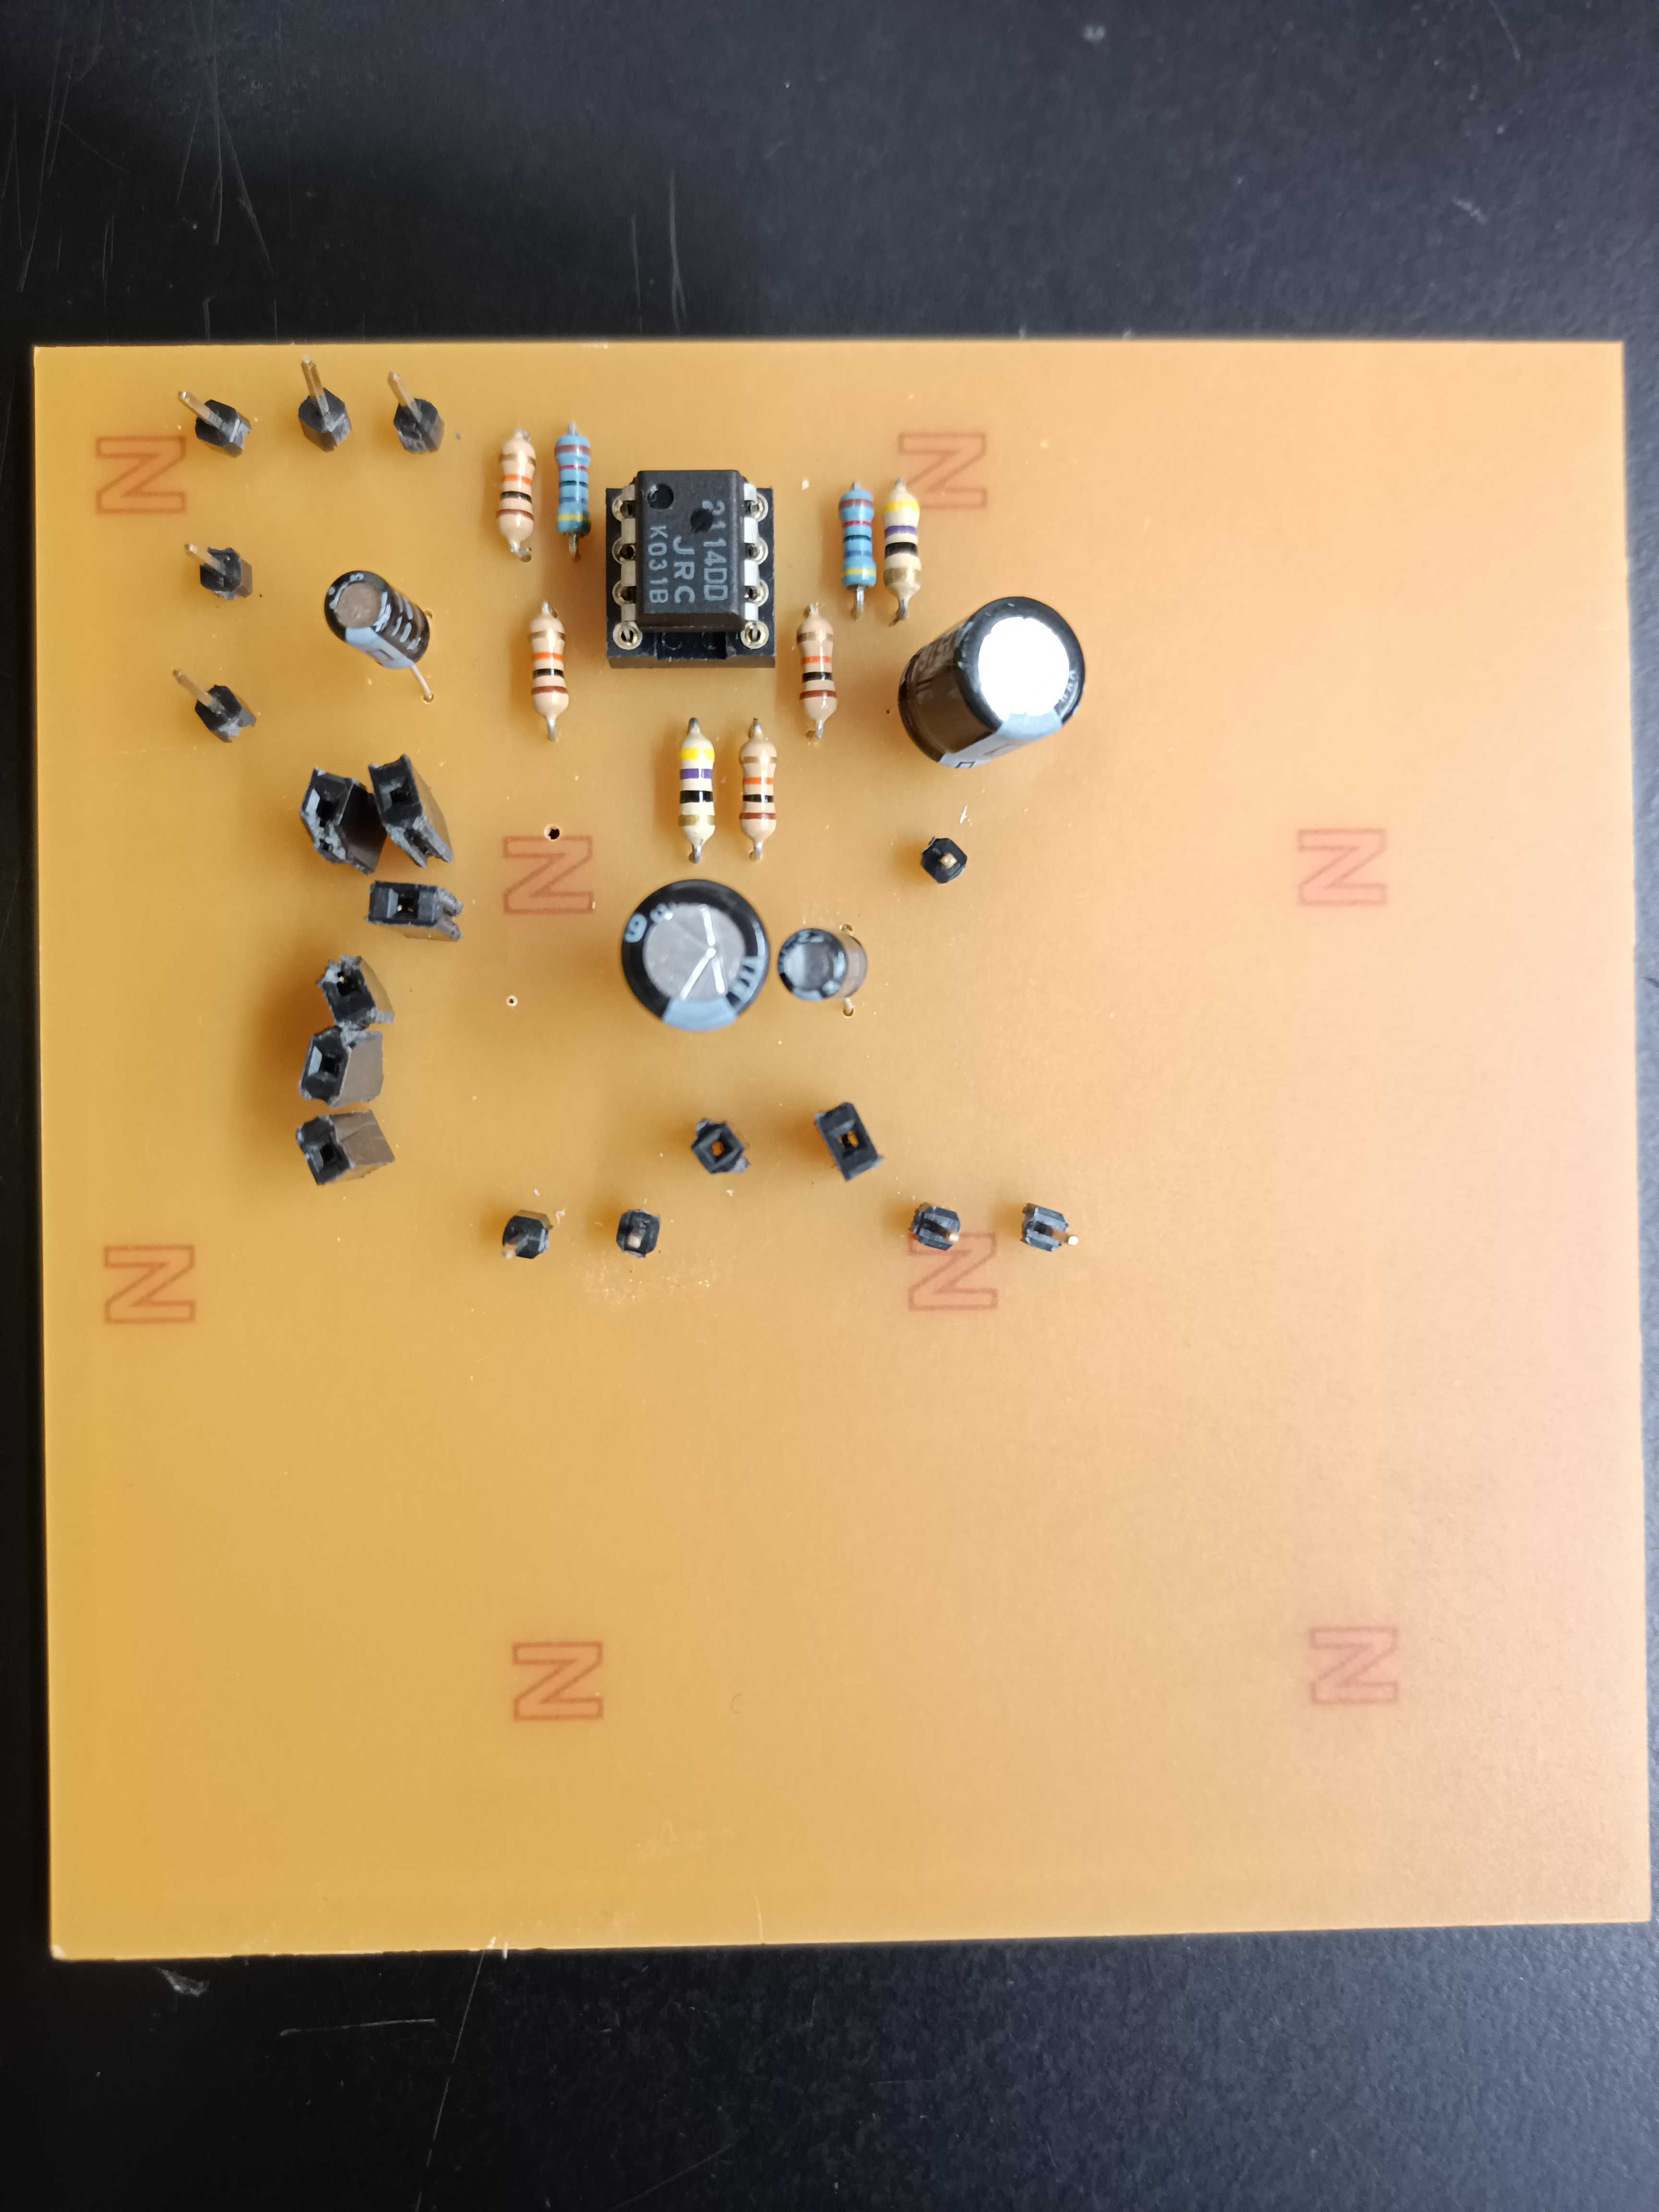
\includegraphics[width=8cm]{use/5.jpg}
		\caption{2号機アンテナの写真}
		\label{fig:s_4}
	\end{minipage}
	\begin{minipage}[b]{0.5\linewidth}
		\centering
		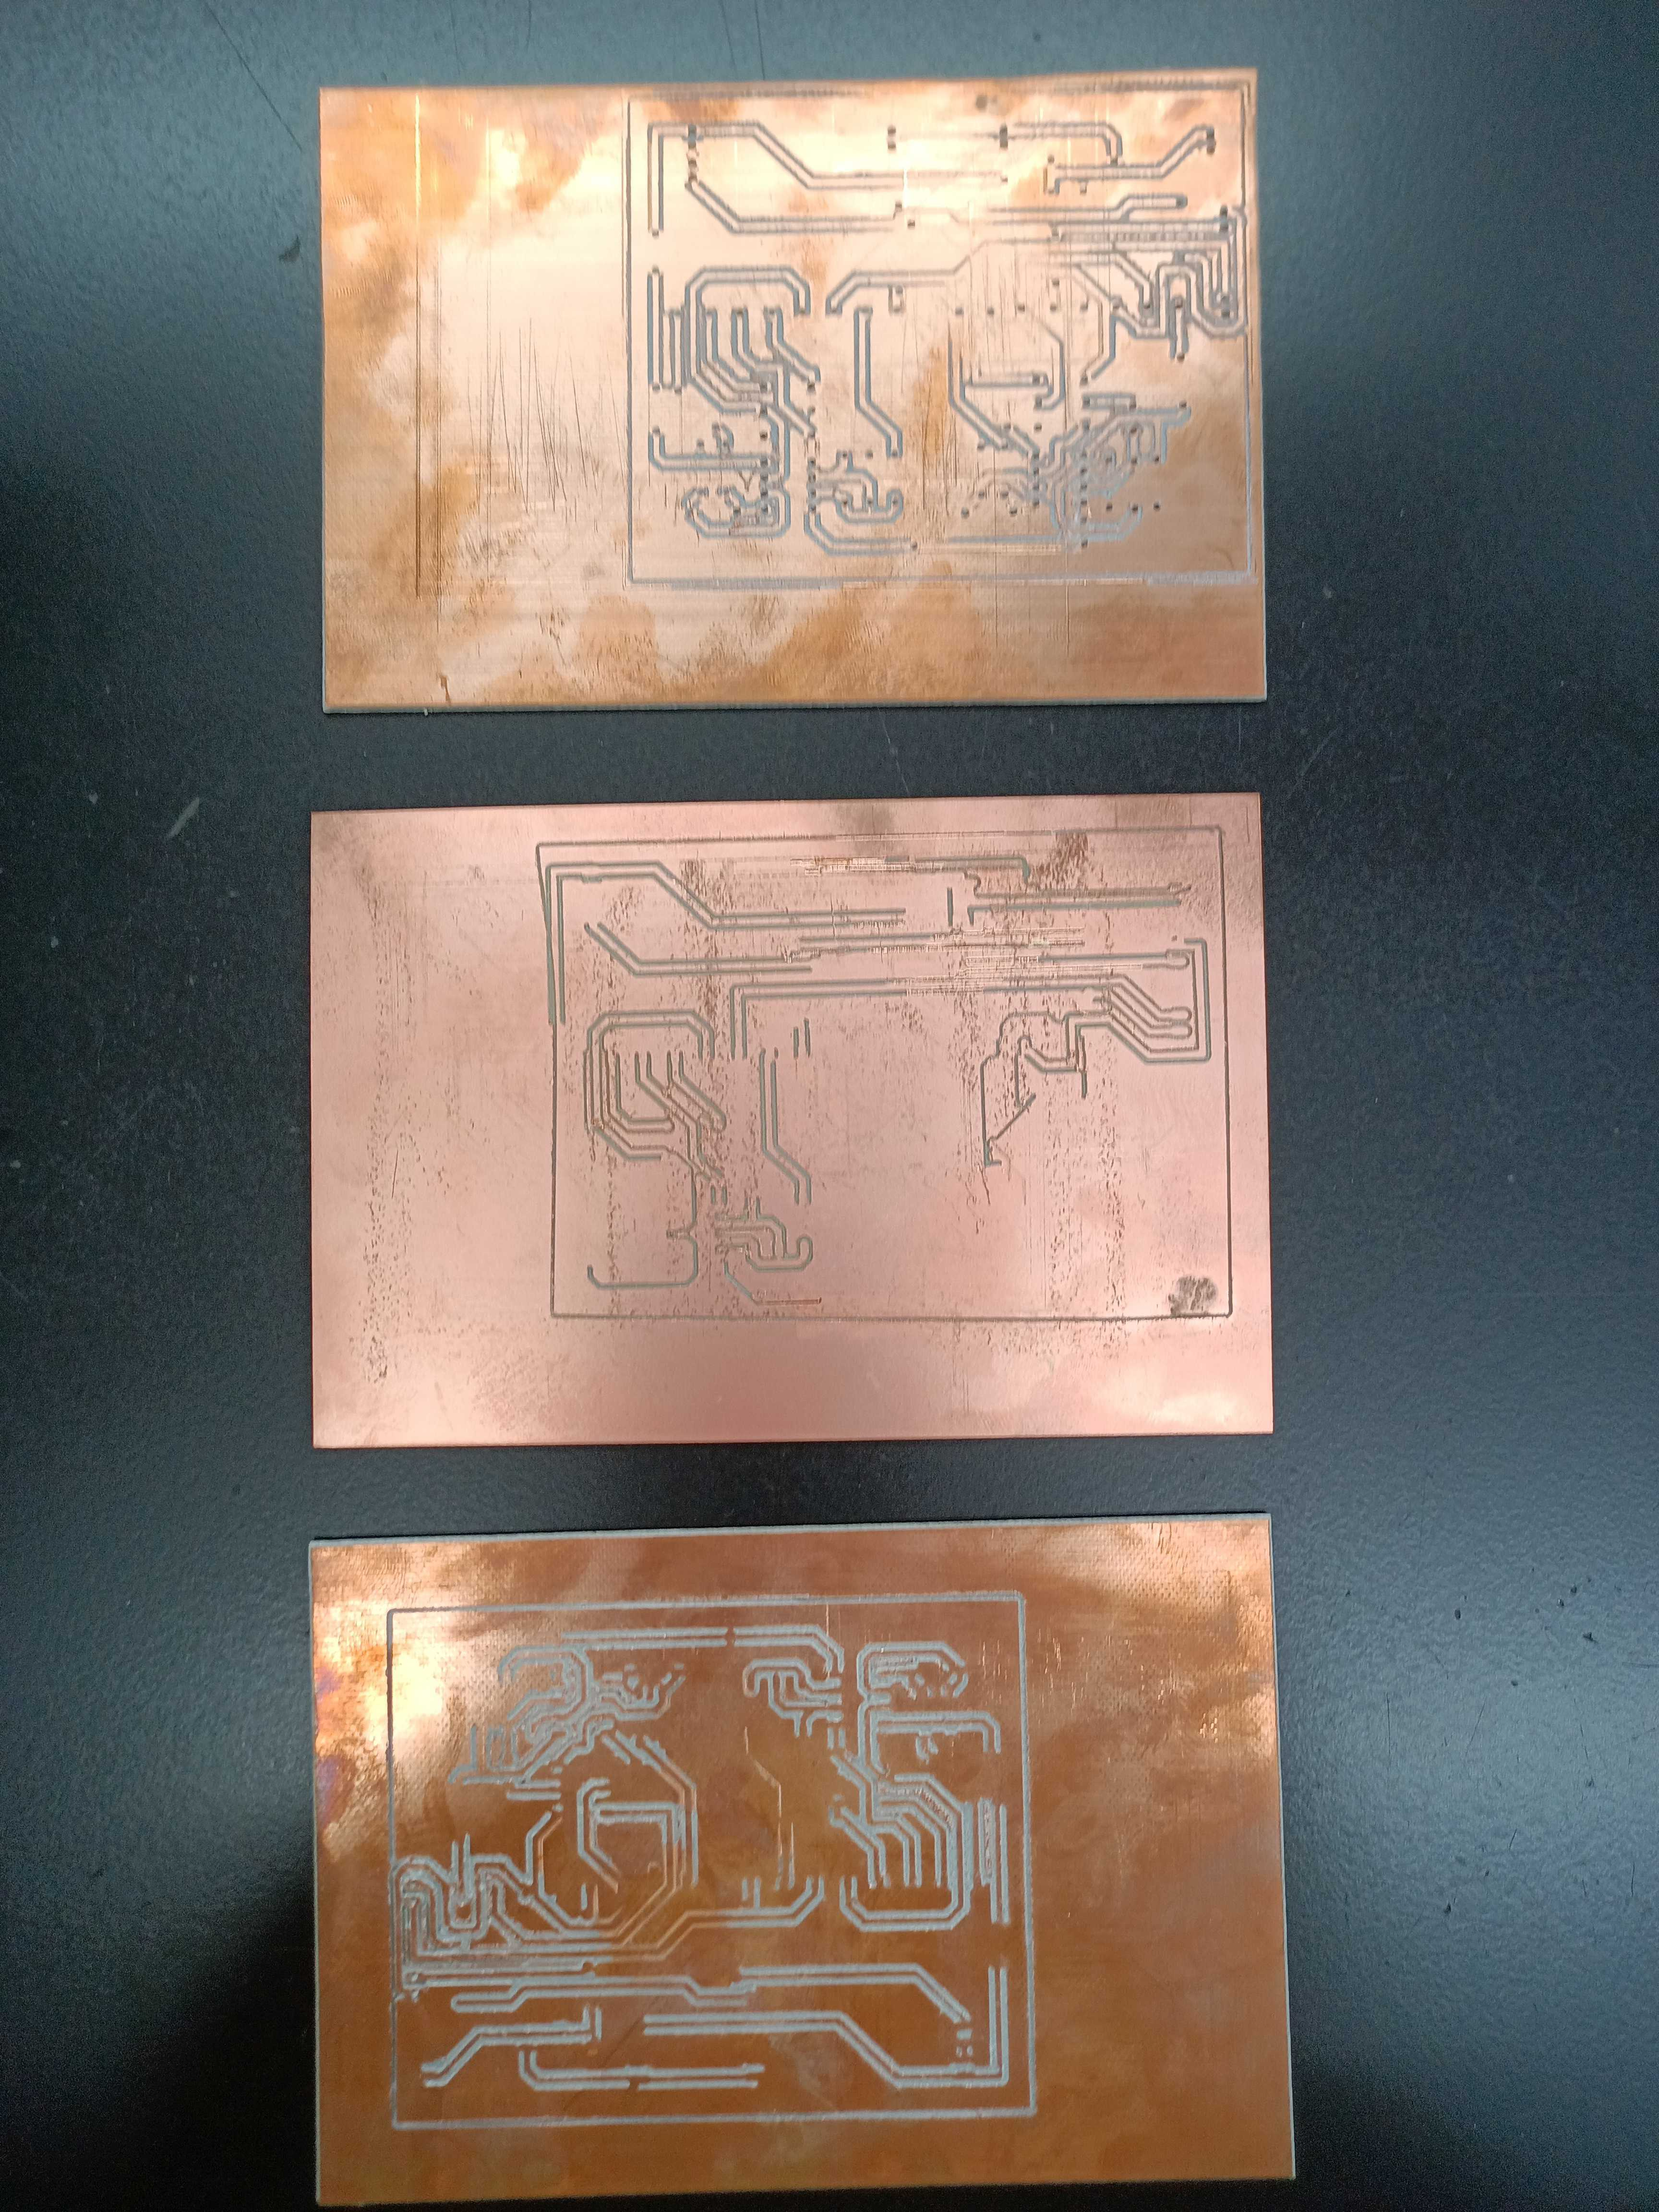
\includegraphics[width=8cm]{use/6.jpg}
		\caption{3号機アンテナの写真}
		\label{fig:s_5}
	\end{minipage}
\end{figure}

\begin{figure}[H]
	\begin{minipage}[b]{0.5\linewidth}
		\centering
		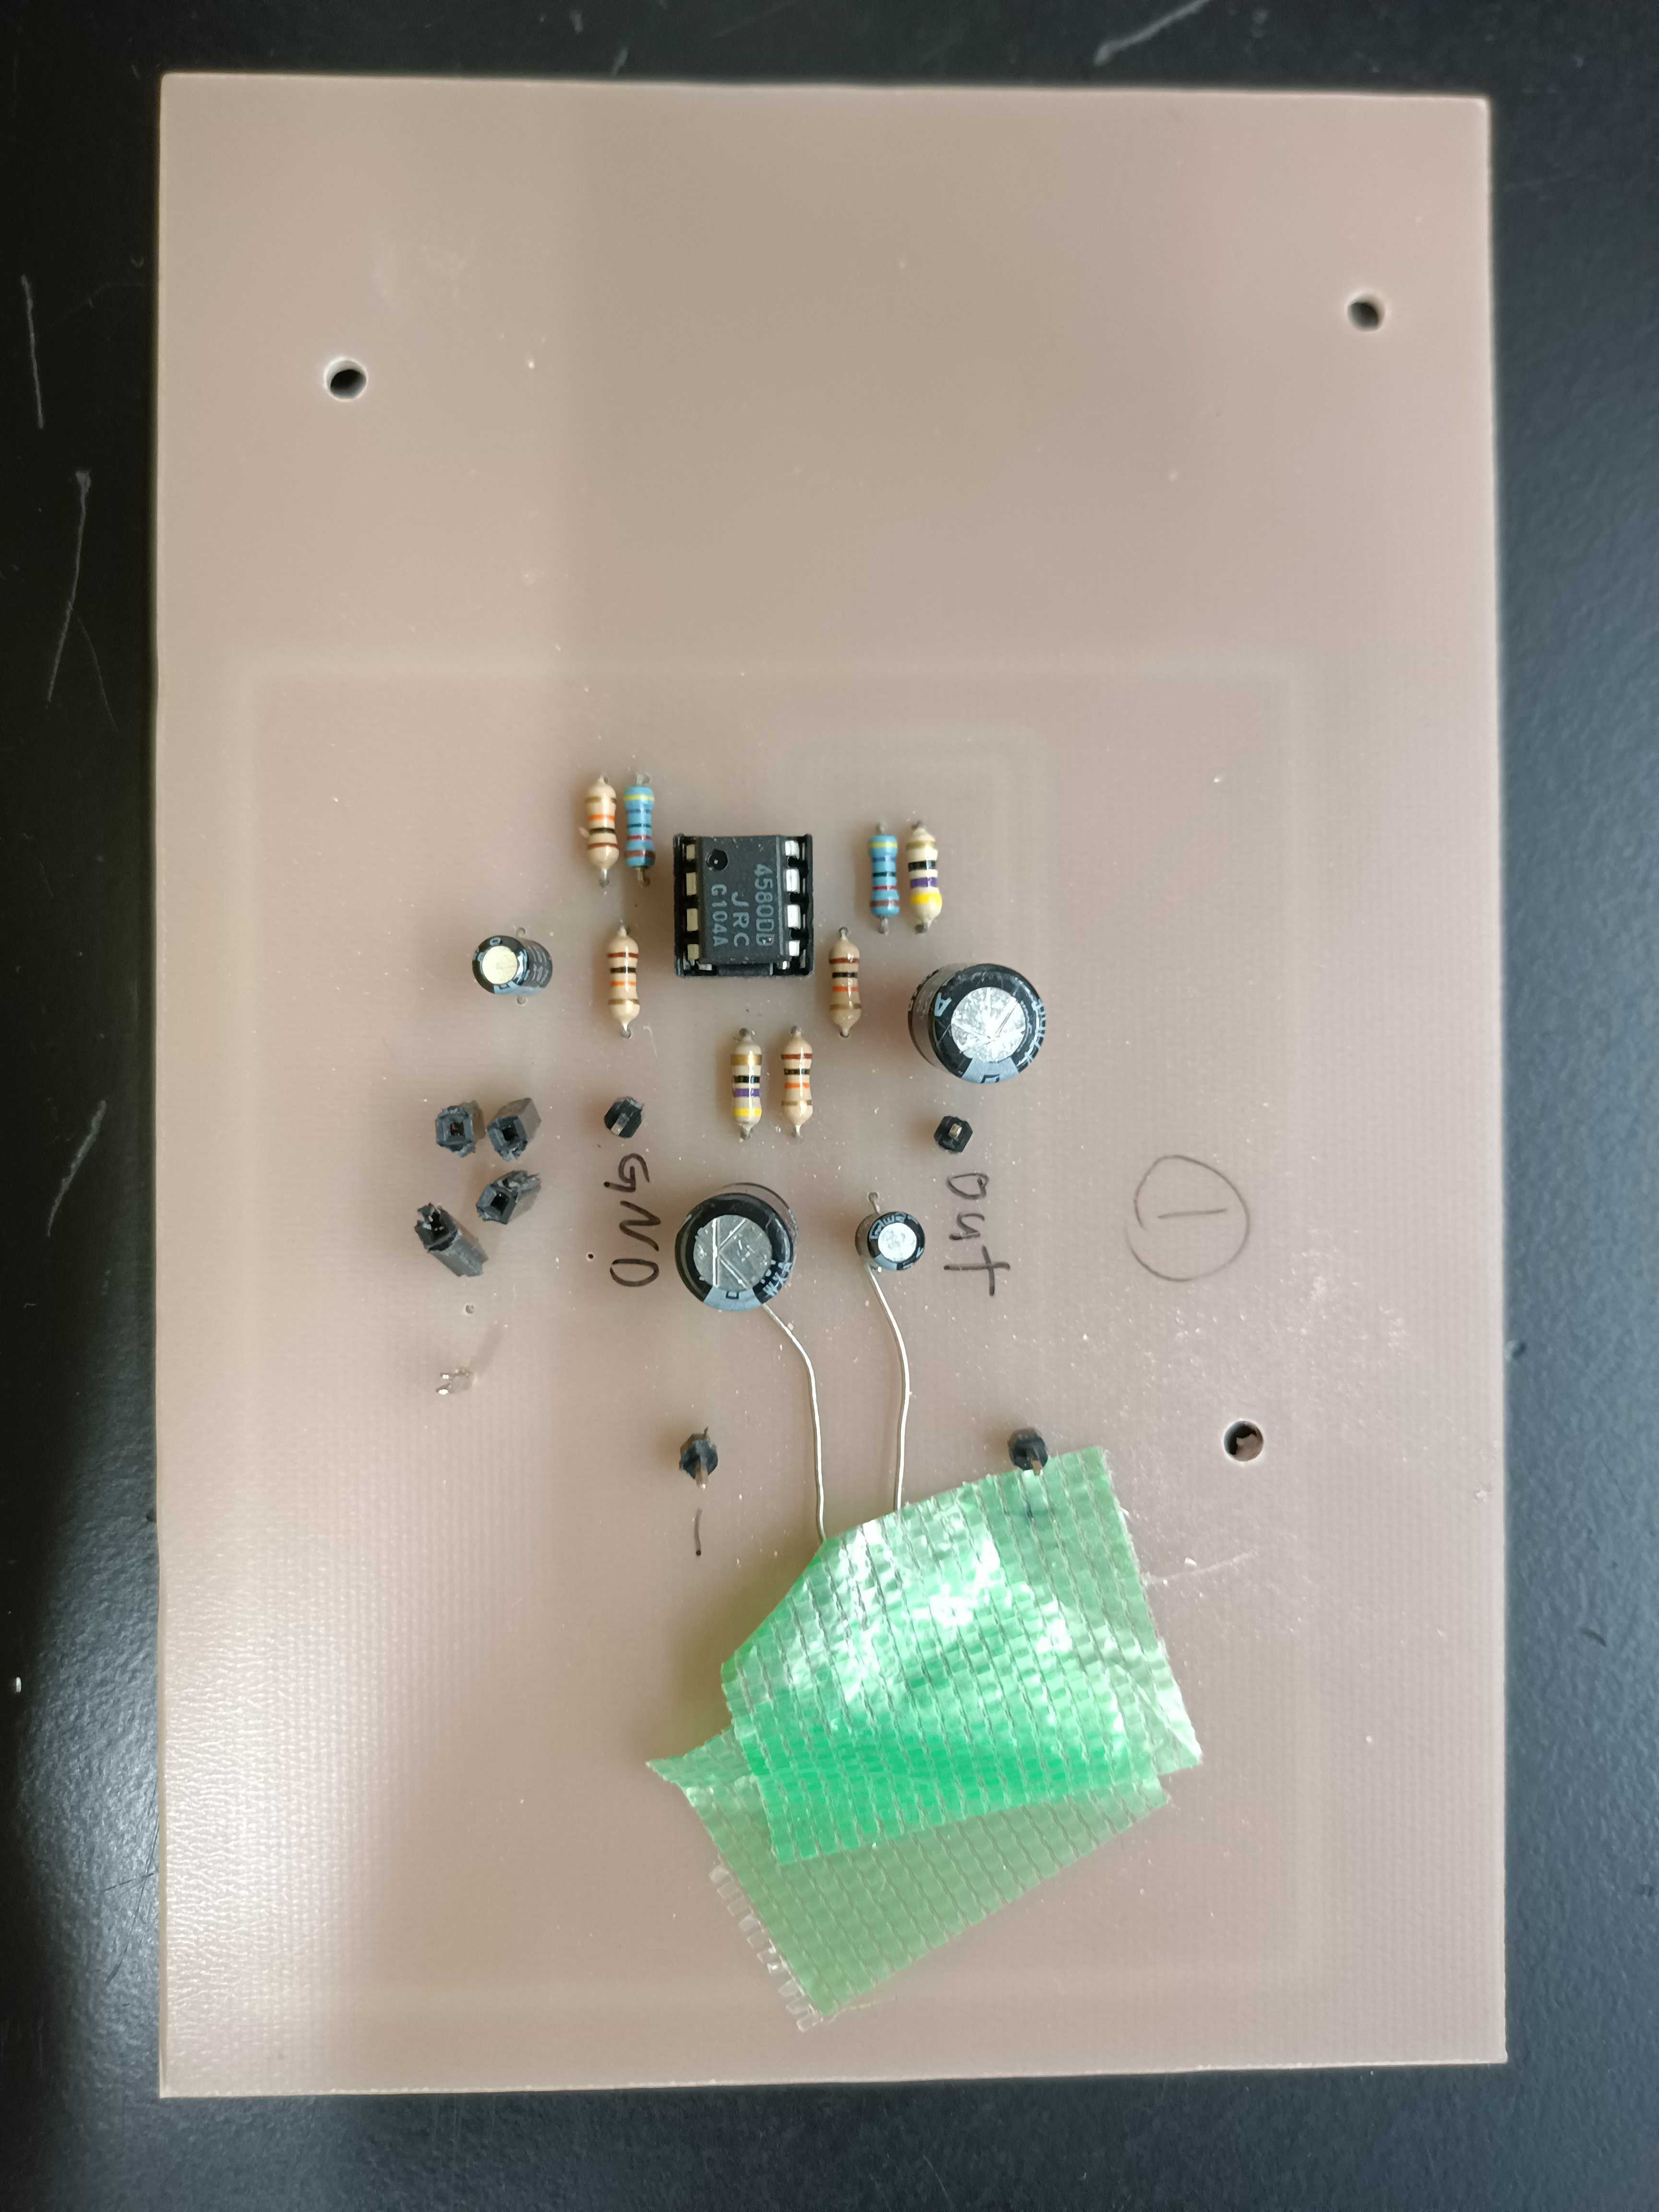
\includegraphics[width=8cm]{use/2.jpg}
		\caption{2号機アンテナの写真}
		\label{fig:s_6}
	\end{minipage}
	\begin{minipage}[b]{0.5\linewidth}
		\centering
		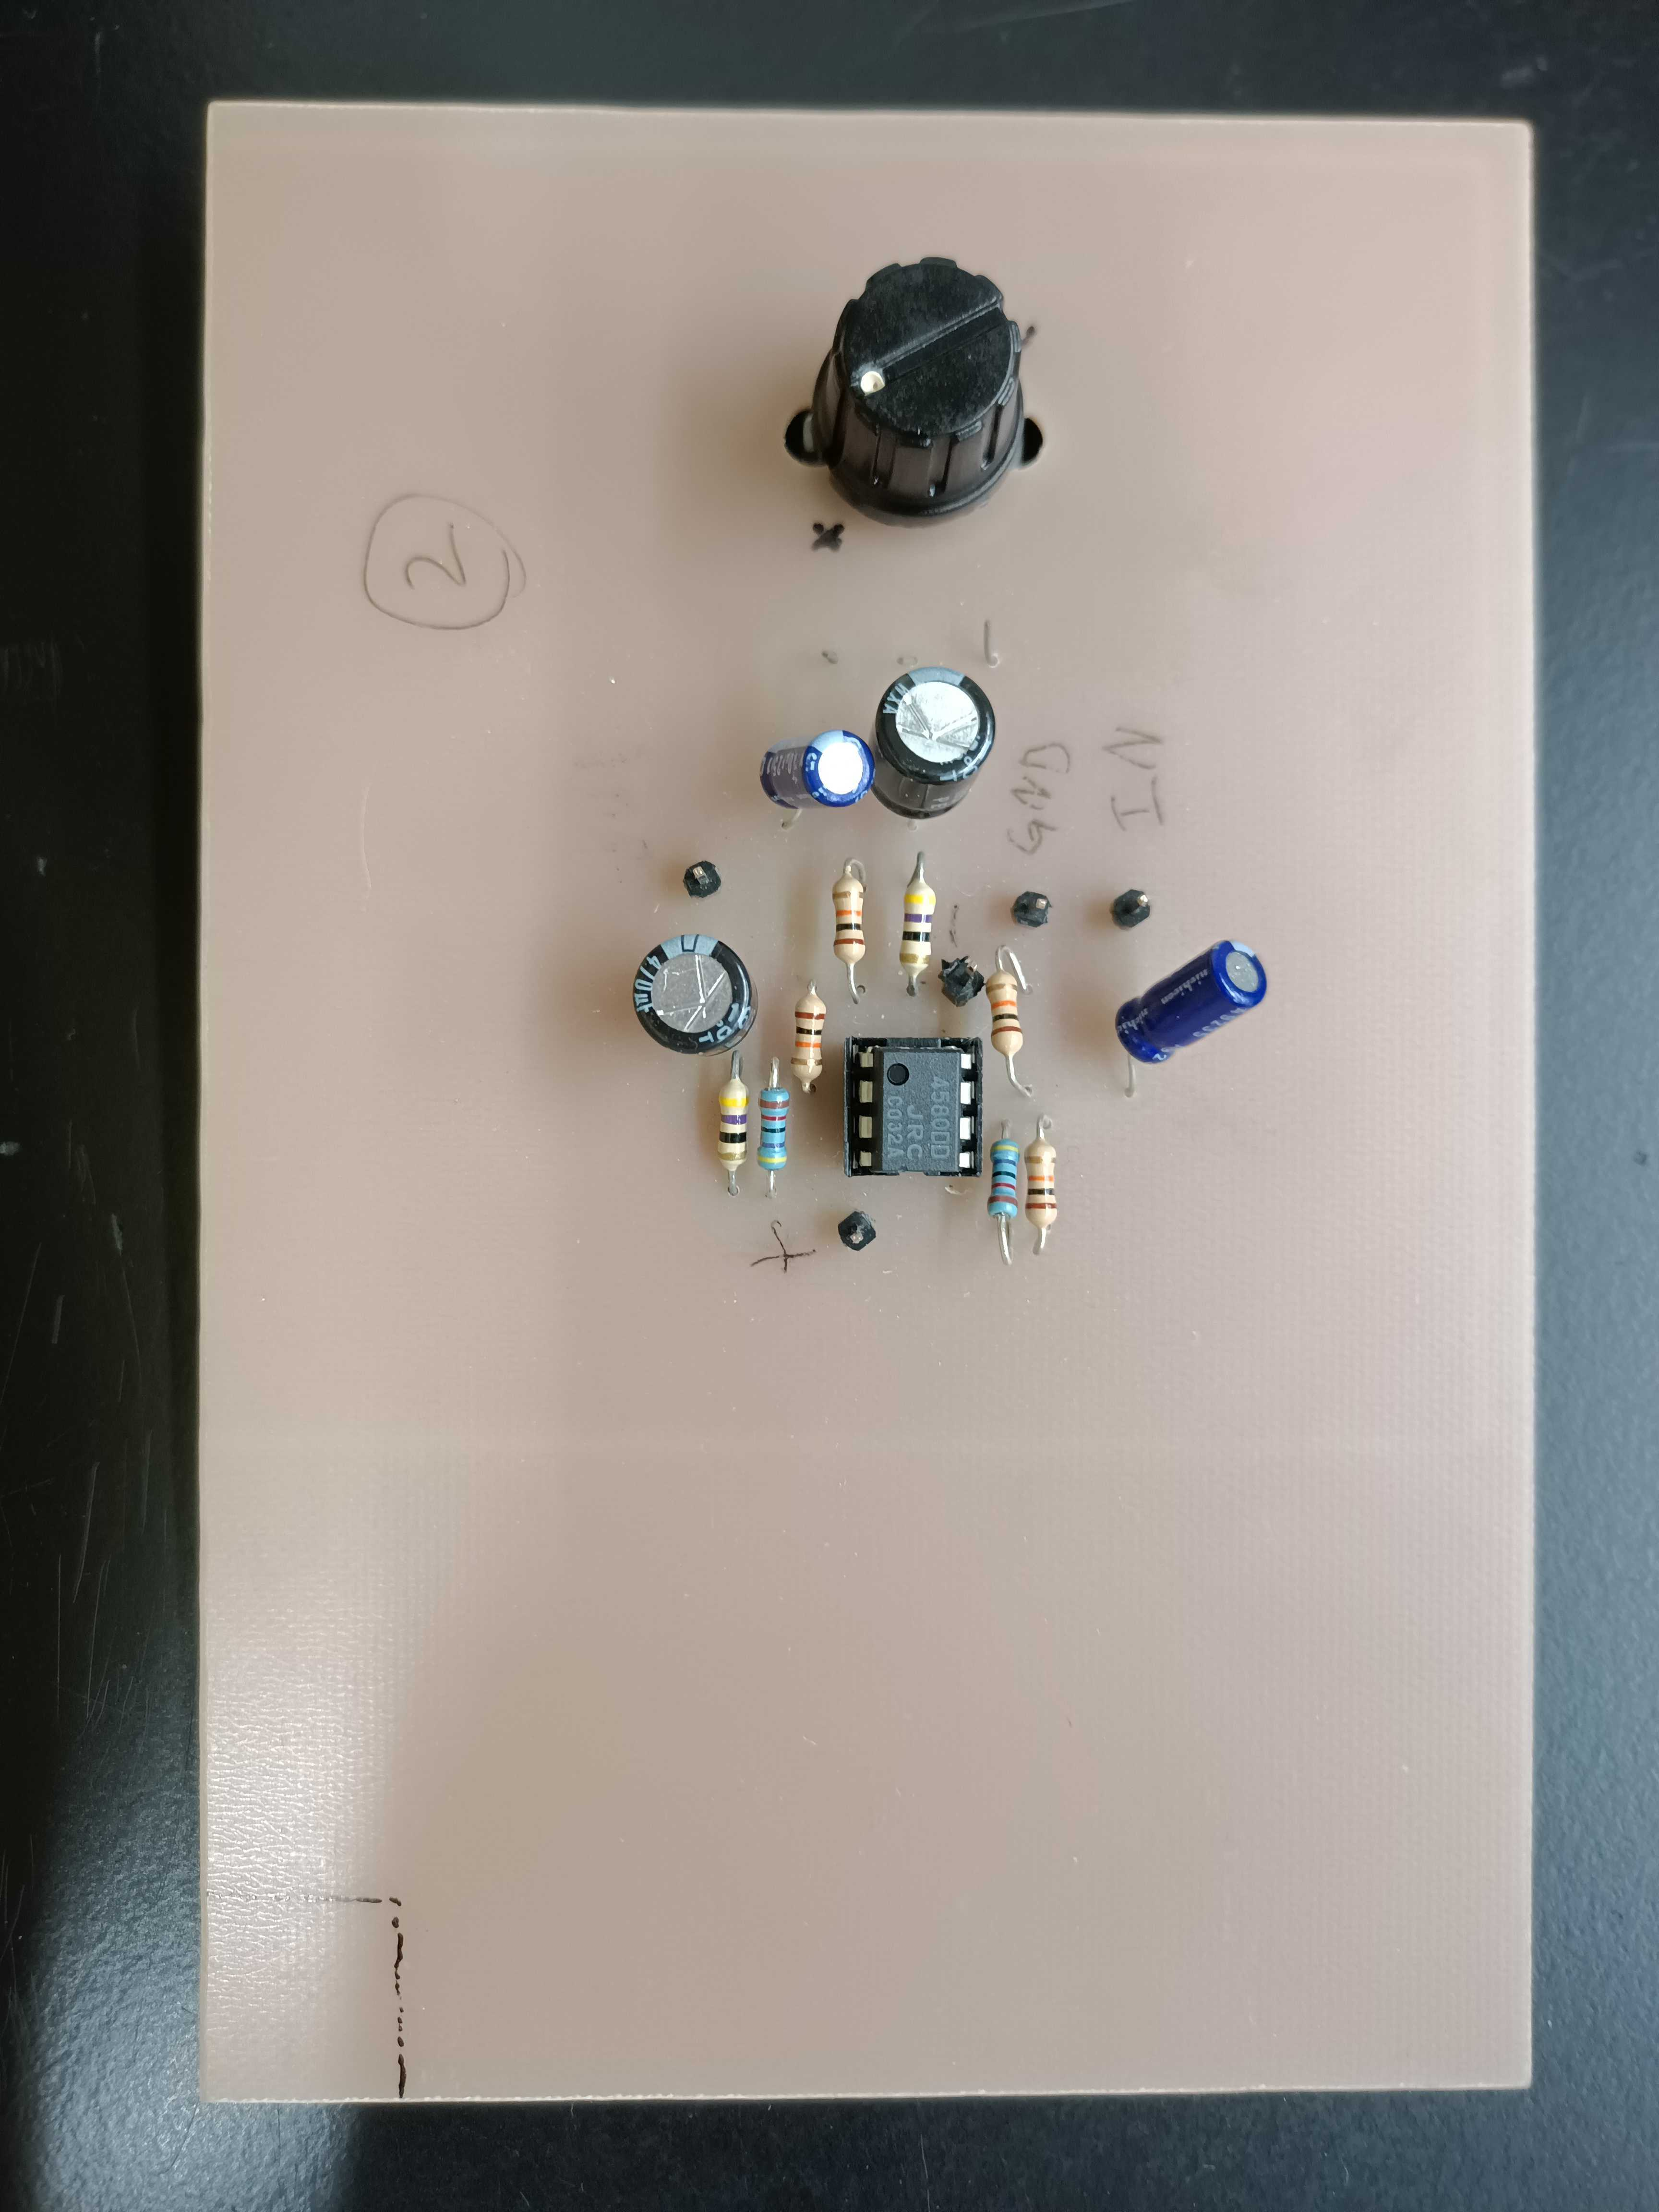
\includegraphics[width=8cm]{use/3.jpg}
		\caption{3号機アンテナの写真}
		\label{fig:s_7}
	\end{minipage}
\end{figure}

\end{document}
